\renewcommand*{\arraystretch}{1.1}

\noindent\begin{tabularx}{17cm}{|p{1.95cm}|X|}
	\hline
	workload    & Interactive / complex \\ \hline
%
	query       & 12 \\ \hline
%
	title       & Expert search \\ \hline
%
    pattern     & \hfill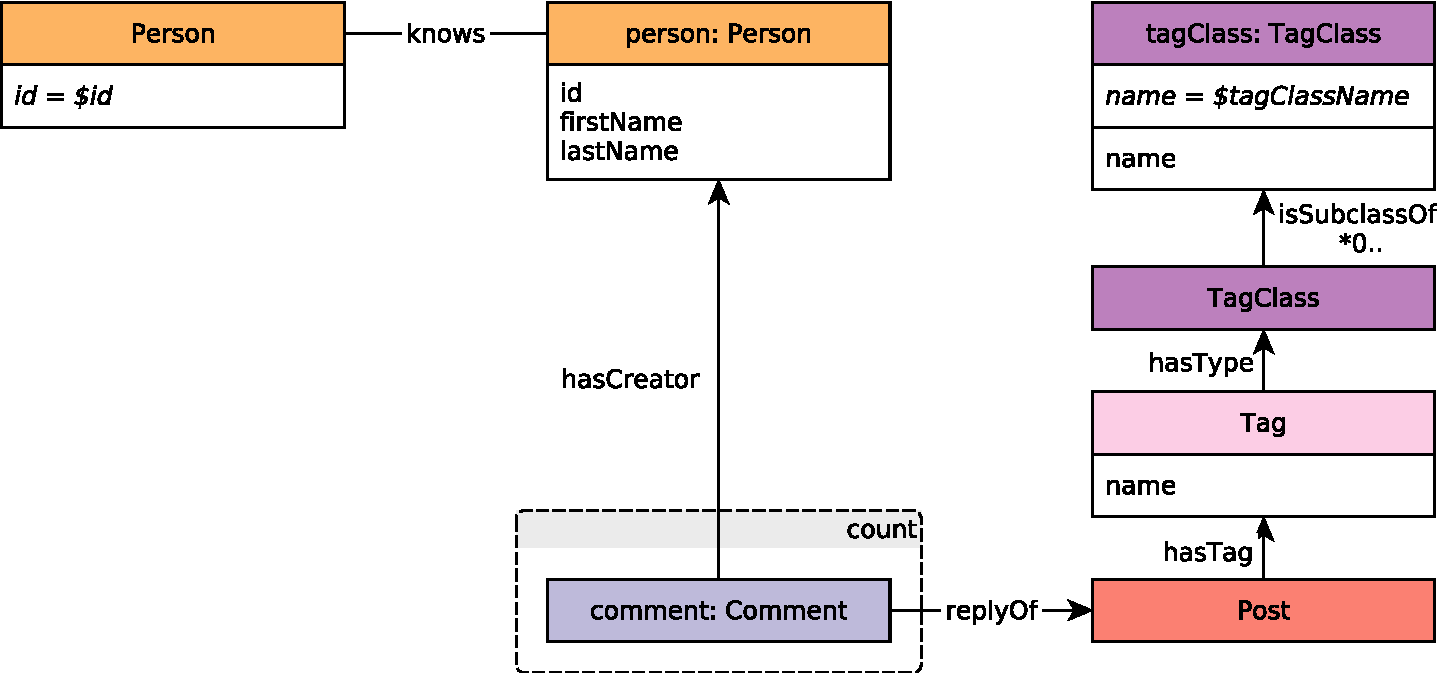
\includegraphics[scale=\patternscale,margin=0cm .2cm]{patterns/interactive-complex-read-12}\hfill\vadjust{} \\ \hline
%
	description & Given a start Person, find the Comments that this Person's friends made
in reply to Posts, considering only those Comments that are immediate
(1-hop) replies to Posts, not the transitive (multi-hop) case. Only
consider Posts with a Tag in a given TagClass or in a descendent of that
TagClass. Count the number of these reply Comments, and collect the Tags
(with valid tag class) that were attached to the Posts they replied to.
Return Persons with at least one reply, the reply count, and the
collection of Tags.
 \\ \hline
	
%
	parameters  &
	\vspace{1.1ex}{\begin{tabularx}{14.2cm}{|c|M|m{2cm}|Y|} \hline
	\cellcolor{black!70} \color{white} $\mathsf{1}$ & \varname{Person.id} & \cellcolor{gray!20} \vartype{ID} &  \\ \hline
	\cellcolor{black!70} \color{white} $\mathsf{2}$ & \varname{TagClass.name} & \cellcolor{gray!20} \vartype{String} &  \\ \hline
	\end{tabularx}}\vspace{1.1ex} \\ \hline
%
	result      &
	\vspace{1.1ex}{\begin{tabularx}{14.2cm}{|c|M|m{2cm}|Y|} \hline
	\cellcolor{black!70} \color{white} $\mathsf{1}$ & \varname{Person.id} & \cellcolor{gray!20} \vartype{ID} &  \\ \hline
	\cellcolor{black!70} \color{white} $\mathsf{2}$ & \varname{Person.firstName} & \cellcolor{gray!20} \vartype{String} &  \\ \hline
	\cellcolor{black!70} \color{white} $\mathsf{3}$ & \varname{Person.lastName} & \cellcolor{gray!20} \vartype{String} &  \\ \hline
	\cellcolor{black!70} \color{white} $\mathsf{4}$ & \varname{\{Tag.name\}} & \cellcolor{gray!20} \vartype{\{String\}} &  \\ \hline
	\cellcolor{black!70} \color{white} $\mathsf{5}$ & \varname{count} & \cellcolor{gray!20} \vartype{32-bit Integer} & number of reply Comments \\ \hline
	\end{tabularx}}\vspace{1.1ex} \\ \hline
	%
	sort        &
	\vspace{1.1ex}{\begin{tabular}{|c|l|c|} \hline
	\cellcolor{black!70} \color{white} $\mathsf{1}$ & \varname{count} & \cellcolor{gray!20} $\desc$ \\ \hline
	\cellcolor{black!70} \color{white} $\mathsf{2}$ & \varname{Person.id} & \cellcolor{gray!20} $\asc$ \\ \hline
	\end{tabular}}\vspace{1.1ex} \\ \hline
	%
	limit       & 20 \\ \hline
	%
	%
\end{tabularx}